\documentclass{standalone}
%% recommended packages

%% more packages 
\usepackage{amsmath, tikz} % for table, equations, and flow chart figure (respectively)
\usetikzlibrary{fit, positioning, shapes} % for flow chart figure


\usepackage{Sweave}
\begin{document}

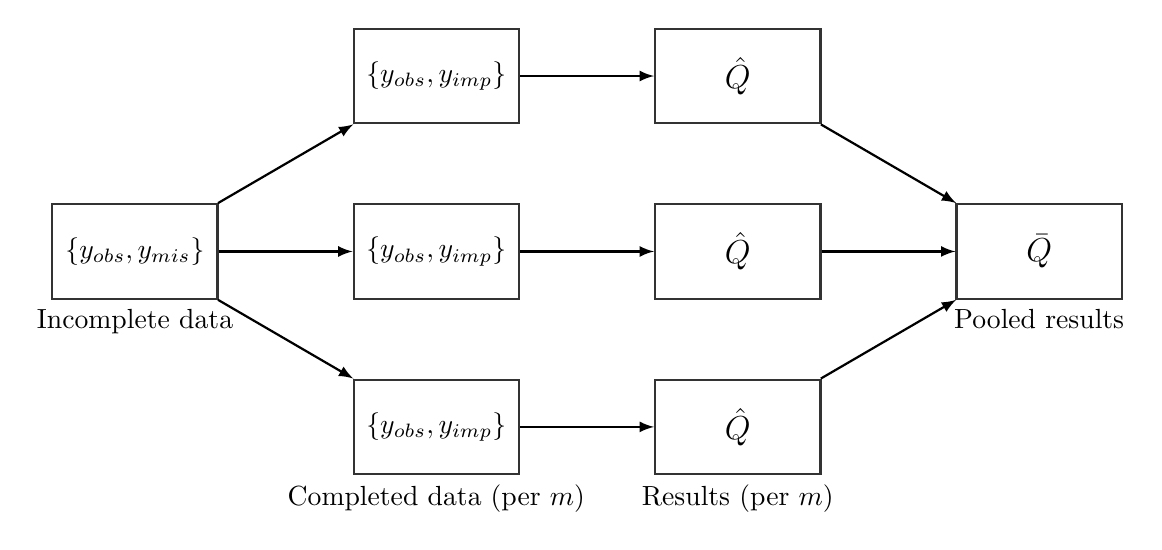
\begin{tikzpicture}
\tikzstyle{main}=[rectangle, minimum width = 21mm, minimum height = 12mm, thick, draw =black!80, node distance = 17mm]
\tikzstyle{connect}=[draw, -latex, thick]
\node[main, fill = white!100] (data) [label=below:Incomplete data] {$\{y_{obs}, y_{mis}\}$};
\node[main] (mids) [right=of data] { $\{y_{obs}, y_{imp}\}$};
\node[main] (mids2) [above=10mm of mids] {$\{y_{obs}, y_{imp}\}$ };
\node[main] (mids3) [below=10mm of mids,label=below: Completed data (per $m$)] { $\{y_{obs}, y_{imp}\}$};
\node[main] (mira) [right=of mids] {\large $\hat{Q}$};
\node[main] (mira2) [above=10mm of mira] {\large $\hat{Q}$ };
\node[main] (mira3) [below=10mm of mira,label=below: Results (per $m$)] {\large $\hat{Q}$ };
\node[main, fill = white!100] (mipo) [right=of mira,label=below:Pooled results] {\large $\bar{Q}$ };
\path (data) edge [connect] (mids)
      (data) edge [connect] (mids2)
      (data) edge [connect] (mids3)
      (mids) edge [connect] (mira)
      (mids2) edge [connect] (mira2)
      (mids3) edge [connect] (mira3)
		  (mira) edge [connect] (mipo)
		  (mira2) edge [connect] (mipo)
		  (mira3) edge [connect] (mipo);
\end{tikzpicture}
%\caption{Scheme of the main steps in multiple imputation \citep[$m = 3$; adapted from][\S~1.4.1]{buur18}. {\footnotesize Missing data in dataset $Y$ is `imputed' (i.e., filled in) $m$ times. The imputed data is combined with the observed data ($Y_{obs}$) to create $m$ completed datasets. On each completed dataset, the analysis of scientific interest (or `substantive model') is performed. The quantity of scientific interest (e.g., a regression coefficient) is denoted with $Q$. Since $Q$ is estimated on each completed dataset, $m$ separate $\hat{Q}$-values are obtained. These $m$ values are combined into a single pooled estimate $\bar{Q}$. $\{y_{obs}, y_{mis}\}$ }} 


\end{document}
